%%%%%%%%%%%%%%%%%%%%%%%%%%%%%%%%%%%%%%%%%%%%%%%%%%%%%%%%%%%%
%%  This Beamer template was created by Cameron Bracken.
%%  Anyone can freely use or modify it for any purpose
%%  without attribution.
%%
%%  Last Modified: January 9, 2009
%%

\documentclass[xcolor=x11names,compress]{beamer}

%% General document %%%%%%%%%%%%%%%%%%%%%%%%%%%%%%%%%%
\usepackage{graphicx}
\usepackage{tikz}
\usepackage[canadian]{babel}
\usepackage[utf8]{inputenc}
\usepackage{amsmath,amssymb}
\usepackage{mathtools}
\usepackage[ruled,vlined,linesnumbered]{algorithm2e}
\usepackage{epstopdf}
\usepackage{hyperref}
\usepackage[export]{adjustbox}
\usepackage{animate}
\usepackage{minted}
\usepackage{xcolor}
\usepackage{pgfplots}
\usetikzlibrary{calc}
\graphicspath{{img/}}
%%%%%%%%%%%%%%%%%%%%%%%%%%%%%%%%%%%%%%%%%%%%%%%%%%%%%%

\DeclareMathOperator*{\argmax}{arg\,max}
\DeclareMathOperator*{\argmin}{arg\,min}
%% Beamer Layout %%%%%%%%%%%%%%%%%%%%%%%%%%%%%%%%%%
\useoutertheme[subsection=false,shadow]{miniframes}
\useinnertheme{default}
\usefonttheme{serif}
\usepackage{palatino}
\urlstyle{same}
\setbeamerfont{title like}{shape=\scshape}
\setbeamerfont{frametitle}{shape=\scshape}

\setbeamercolor*{lower separation line head}{bg=DeepSkyBlue4} 
\setbeamercolor*{normal text}{fg=black,bg=white} 
\setbeamercolor*{alerted text}{fg=red} 
\setbeamercolor*{example text}{fg=black} 
\setbeamercolor*{structure}{fg=black} 
 
\setbeamercolor*{palette tertiary}{fg=black,bg=black!10} 
\setbeamercolor*{palette quaternary}{fg=black,bg=black!10} 

\renewcommand{\(}{\begin{columns}}
\renewcommand{\)}{\end{columns}}
\newcommand{\<}[1]{\begin{column}{#1}}
\renewcommand{\>}{\end{column}}
\setbeamertemplate{navigation symbols}{}

\setbeamerfont{footline}{size=\fontsize{6}{0}\selectfont}
\setbeamercolor{footline}{fg=black!50}

\setbeamertemplate{footline}{
	\parbox{\paperwidth}{\hspace*{5pt}\url{http://www.cs.toronto.edu/~frossard}\hfill
		\insertframenumber/\inserttotalframenumber\hspace*{5pt}}
	}
\usemintedstyle{tango}
%%%%%%%%%%%%%%%%%%%%%%%%%%%%%%%%%%%%%%%%%%%%%%%%%%


\begin{document}


%%%%%%%%%%%%%%%%%%%%%%%%%%%%%%%%%%%%%%%%%%%%%%%%%%%%%%
%%%%%%%%%%%%%%%%%%%%%%%%%%%%%%%%%%%%%%%%%%%%%%%%%%%%%%
\section{\scshape Introduction}
\begin{frame}
\title{Introduction to Machine Learning}
\subtitle{Course Introduction}
\author{
	Davi Frossard\\
	{\it Federal University of Espirito Santo \\ University of Toronto}\\
}
\date{
    \vspace{-3.5em}\\
    \includegraphics[width=0.6\columnwidth]{ml.png}\\[-1ex]
    {\tiny Credit: {\itshape \url{https://www.lexalytics.com/technology/machine-learning}}}
    \\
	\today
}
\titlepage
\end{frame}

%%%%%%%%%%%%%%%%%%%%%%%%%%%%%%%%%%%%%%%%%%%%%%%%%%%%%%
%%%%%%%%%%%%%%%%%%%%%%%%%%%%%%%%%%%%%%%%%%%%%%%%%%%%%%
\begin{frame}{Summary}
\tableofcontents
\end{frame}

%%%%%%%%%%%%%%%%%%%%%%%%%%%%%%%%%%%%%%%%%%%%%%%%%%%%%%
%%%%%%%%%%%%%%%%%%%%%%%%%%%%%%%%%%%%%%%%%%%%%%%%%%%%%%
\subsection{Course Structure}
\begin{frame}{Course Structure}
\begin{itemize}
\item Lectures
\item Coding Tutorials
\item Challenges
\begin{itemize}
\item Kaggle in Class
\end{itemize}
\item Online Resources
\end{itemize}
\end{frame}

%%%%%%%%%%%%%%%%%%%%%%%%%%%%%%%%%%%%%%%%%%%%%%%%%%%%%%
%%%%%%%%%%%%%%%%%%%%%%%%%%%%%%%%%%%%%%%%%%%%%%%%%%%%%%
\subsection{Course Content}
\begin{frame}{Content \tiny{Tentative - In chronological order}}
\begin{itemize}
\item K Nearest Neighbors

\item Simple \& Multiple Linear Regression
    \begin{itemize}
    \item Vectorization
    \item Gradient Descent
    \end{itemize}

\item TensorFlow

\item Logistic Regression

\item Fully Connected Neural Networks
    \begin{itemize}
    \item Backpropagation
    \item Overfitting
    \item Initialization
    \end{itemize}

\item Convolutional Neural Networks
    \begin{itemize}
    \item Guided Backpropagation
    \end{itemize}
    
\item Recurrent Neural Networks
    \begin{itemize}
    \item Vanishing Gradient
    \item Long Short Term Memory
    \end{itemize}
\end{itemize}
\end{frame}

%%%%%%%%%%%%%%%%%%%%%%%%%%%%%%%%%%%%%%%%%%%%%%%%%%%%%%
%%%%%%%%%%%%%%%%%%%%%%%%%%%%%%%%%%%%%%%%%%%%%%%%%%%%%%
\subsection{Prerequisites}
\begin{frame}{Prerequisites}
\begin{itemize}
\item Linear Algebra
    \begin{itemize}
    \item Scalar and Vector Operators
    \item Eigenvalues \& Eigenvectors
    \end{itemize}

\item Calculus
    \begin{itemize}
    \item Derivatives \& Gradients
    \item Integrals
    \item Function Minimization
    \end{itemize}

\item Probability
    \begin{itemize}
    \item Distributions
    \item Random Variables
    \item Expectation
    \item Independence
    \end{itemize}
\end{itemize}
\end{frame}

%%%%%%%%%%%%%%%%%%%%%%%%%%%%%%%%%%%%%%%%%%%%%%%%%%%%%%
%%%%%%%%%%%%%%%%%%%%%%%%%%%%%%%%%%%%%%%%%%%%%%%%%%%%%%
\section{\scshape Machine Learning}
\begin{frame}{Machine Learning}
	\begin{itemize}
		\item Problems hard to solve programmatically:
		\begin{itemize}
			\item Recognize a face.
			\item Recommend relevant ads.
			\item Identify spam email.
			\item \textbf{Decide the next move in a game of Go.}
		\end{itemize}	
	\end{itemize}
\end{frame}


%%%%%%%%%%%%%%%%%%%%%%%%%%%%%%%%%%%%%%%%%%%%%%%%%%%%%%
%%%%%%%%%%%%%%%%%%%%%%%%%%%%%%%%%%%%%%%%%%%%%%%%%%%%%%
\subsection{\scshape Minimax Algorithm}
\begin{frame}{Minimax}
	\begin{itemize}
		\item Minimize the maximum reward
	\end{itemize}
	\begin{center}
		 \newcommand*\redone{}
		 \newcommand*\blacktwo{}
		 \newcommand*\blackthree{}
		 \only<8->{\renewcommand*\redone{red}}
		 \only<9->{\renewcommand*\blacktwo{black}}
		 \only<10->{\renewcommand*\blackthree{black}}
		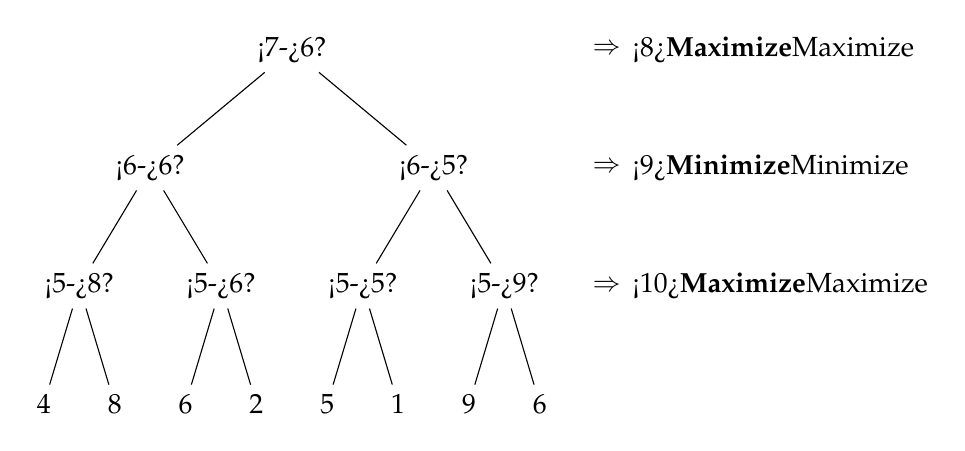
\begin{tikzpicture}[level distance=1.5cm,
		level 1/.style={sibling distance=3.6cm},
		level 2/.style={sibling distance=1.8cm},
		level 3/.style={sibling distance=0.9cm}]
		\uncover<1->{\node (Root) [\redone] {\alt<7->{6}{?}}
		child [\redone] {	node {\alt<6->{6}{?}}
			child [\blacktwo] {	node {\alt<5->{8}{?}}
				child {	node {4} }
				child {	node {8} }
			}
			child { node {\alt<5->{6}{?}}
				child { node {6} }
				child [\blackthree] {	node {2} }
			}
		}
		child {	node {\alt<6->{5}{?}}
			child {	node {\alt<5->{5}{?}}
				child { node {5} }
				child {	node {1} }
			}
			child { node {\alt<5->{9}{?}}
				child {	node {9} }
				child {	node {6} }
			}
		};}
		\begin{scope}[every node/.style={right}]
		\uncover<2->{\path (Root     -| Root-2-2) ++(1cm,0) node {$\Rightarrow$} ++(5mm,0) node {\alt<8>{\textbf{Maximize}}{Maximize}};}
		\uncover<3->{\path (Root-1   -| Root-2-2) ++(1cm,0) node {$\Rightarrow$} ++(5mm,0) node {\alt<9>{\textbf{Minimize}}{Minimize}};}
		\uncover<4->{\path (Root-1-1 -| Root-2-2) ++(1cm,0) node {$\Rightarrow$} ++(5mm,0) node {\alt<10>{\textbf{Maximize}}{Maximize}};}
		\end{scope}
		\end{tikzpicture}
	\end{center}
\end{frame}

%%%%%%%%%%%%%%%%%%%%%%%%%%%%%%%%%%%%%%%%%%%%%%%%%%%%%%
%%%%%%%%%%%%%%%%%%%%%%%%%%%%%%%%%%%%%%%%%%%%%%%%%%%%%%
\begin{frame}{Minimax}
	\begin{itemize}
		\item Branching factor of 2 and limited height.
		\item Solution space of $2^{n+1}-1$
		\item Easily tractable.
		\uncover<2->{\item Tic Tac Toe
		\begin{itemize}
			\item Solution space of $9!$
		\end{itemize}}
		\uncover<3->{\item Checkers
		\begin{itemize}
			\item Solution space of $10^{40}$
		\end{itemize}}
		\uncover<4->{\item Chess
		\begin{itemize}
			\item Solution space of $10^{120}$
		\end{itemize}}
		\uncover<5->{\item Go
		\begin{itemize}
			\item Solution space of $\sim2.08\times10^{170}$
			\uncover<6->{\item Need a considerably larger universe to fit a computer able to solve it with brute force.}
		\end{itemize}}
	\end{itemize}
\end{frame}

%%%%%%%%%%%%%%%%%%%%%%%%%%%%%%%%%%%%%%%%%%%%%%%%%%%%%%
%%%%%%%%%%%%%%%%%%%%%%%%%%%%%%%%%%%%%%%%%%%%%%%%%%%%%%
\subsection{\scshape Deep Learning}
\begin{frame}{Deep Learning}
	\begin{itemize}
		\item Decide the next step by detecting patterns in the game.
		\item Learn how to play by playing against humans, then against itself.
		\begin{itemize}
			\item \textbf{Reinforcement Learning}.
		\end{itemize}
		\item Learn to predict current game value ("likelihood of a win") and next move.
		\item AlphaGo beat Lee Sedol, strongest Go player in the world, 4-1 in March 2016.
	\end{itemize}
\end{frame}


%%%%%%%%%%%%%%%%%%%%%%%%%%%%%%%%%%%%%%%%%%%%%%%%%%%%%%
%%%%%%%%%%%%%%%%%%%%%%%%%%%%%%%%%%%%%%%%%%%%%%%%%%%%%%
\begin{frame}{Flavours of Machine Learning}
	\begin{itemize}
		\item Supervised Learning
		\begin{itemize}
			\item Learn by observing labelled data.
		\end{itemize}
		\item Unsupervised Learning
		\begin{itemize}
			\item Learn by extracting useful patterns from unlabelled data.
		\end{itemize}
		\item Reinforcement Learning
		\begin{itemize}
			\item Learn by reward from action.
		\end{itemize}
		\item Semi-supervised Learning
		\begin{itemize}
			\item Mix of supervised and unsupervised approaches.
		\end{itemize}
	\end{itemize}
\end{frame}

%%%%%%%%%%%%%%%%%%%%%%%%%%%%%%%%%%%%%%%%%%%%%%%%%%%%%%
%%%%%%%%%%%%%%%%%%%%%%%%%%%%%%%%%%%%%%%%%%%%%%%%%%%%%%
\begin{frame}{Fields}
	\begin{itemize}
		\item Computer Vision
		\item Natural Language Processing
		\item Economics
		\item Genomic Medicine
		\item $\vdots$
	\end{itemize}
\end{frame}

\end{document}